\section{Student's \(t\)-distribution}

\begin{remark}
  Some discussions in this section are not included in the lecture notes of ENGG2780 but are helpful for understanding. They are marked with \(\circledast\). 
\end{remark}

Previously, we talked about the case when \(\sigma^2\) is known, and with a large sample \(n\), we can find the \((1 - \alpha)\) confidence interval for the mean \(\mu\). Now, if we have an unknown \(\sigma^2\) and a large \(n\) (\(n \geq 30\)), then we have a \(1 - \alpha\) confidence interval for the mean \(\mu\):  
\[
  \overline{x} \pm z_{\frac{\alpha}{2}} \dfrac{s}{\sqrt{n}}, \quad s^2 = \dfrac{\sum_{i = 1}^n (X_i - \overline{X})^2}{n - 1}.
\]

\begin{intuition}
  As \(\sigma^2\) is unknown, we cannot utilize \(Z = \frac{\overline{X} - \mu}{\frac{\sigma}{\sqrt{n}}} \sim \mathcal{N}(0, 1)\) to construct the confidence interval. Instead, we need to analyze the distribution of \(\frac{\overline{X} - \mu}{\frac{S}{\sqrt{n}}}\), where the unbiased sample standard deviation \(S\) is a random variable. 
  
  Here we consider \(X_1, \cdots, X_n\) as independent random variables with a large \(n\). 
  
  \textbf{Case I:} For \(X_i \sim \mathcal{N}(\mu, \sigma^2)\), we have 
  \[
    \frac{\overline{X} - \mu}{\frac{S}{\sqrt{n}}} \sim t(n - 1) \overset{n \to \infty}{\longrightarrow} \mathcal{N}(0, 1)
  \] 
  Then we have 
  \[
    \frac{\overline{X} - \mu}{\frac{S}{\sqrt{n}}} \sim \mathcal{N}(0, 1) \Rightarrow \mathbb{P}\left(-z_{\frac{\alpha}{2}} \leq \frac{\overline{X} - \mu}{\frac{S}{\sqrt{n}}} \leq z_{\frac{\alpha}{2}}\right) = 1 - \alpha
  \] 
  Given a specific sample mean and standard deviation \(\overline{x}, s\), the interval becomes fixed. 
  
  \textbf{Case II:} 
  If the distribution of \(X_i\) is unknown, then based on the Central Limit Theorem, we have 
  \[
    \sqrt{n}(\overline{X} - \mu) \xrightarrow{d} \mathcal{N}(0, \sigma^2). 
  \]
  As \(\frac{\overline{X} - \mu}{\sigma / \sqrt{n}} = \frac{\sqrt{n}(\overline{X} - \mu)}{\sigma} \sim t(n - 1)\), we have 
  \[
    S^2 = \frac{1}{n-1} \sum_{i=1}^{n} (X_i - \overline{X})^2 \overset{P}{\longrightarrow} \sigma^2
  \] 
  Then, from Slutsky's Theorem, we have 
  \[
    \frac{\overline{X} - \mu}{\frac{S}{\sqrt{n}}} = \frac{\sqrt{n}(\overline{X} - \mu)}{S} = Z \sim \mathcal{N}(0, 1)
  \] 
  As \(n\) is large, the distribution of \(\frac{\overline{X} - \mu}{\frac{S}{\sqrt{n}}}\) is assumed to be approximated by \(\mathcal{N}(0, 1)\).
\end{intuition}

However, when \(\sigma\) is unknown and we have a small \(n\), how can we find the confidence interval? This brings us to the Student's \(t\)-distribution.



\subsection{Chi-squared Random Variable}
We first take a look at some normal algebra. 

Suppose we have \(X_1 \sim \text{Normal}(\mu_1, \sigma_1)\) and \(X_2 \sim \text{Normal}(\mu_2, \sigma_2)\), where \(X_1, X_2\) are independent. Then, we have \(X_1 + X_2 \sim \text{Normal}(\mu_1 + \mu_2, \sqrt{\sigma_1^2 + \sigma_2^2})\) and \(X_1 - X_2 \sim \text{Normal}(\mu_1 - \mu_2, \sqrt{\sigma_1^2 + \sigma_2^2})\).

Then, the adjusted sample variance \(S^2\) of two independent \(\text{Normal}(\mu, \sigma)\) samples is 
\[
  \begin{aligned}
    S^2 &= (X_1 - \overline{X})^2 + (X_2 - \overline{X})^2 \\
    &= (X_1 - \dfrac{X_1 + X_2}{2})^2 + (X_2 - \dfrac{X_1 + X_2}{2})^2 \\
    &= \left(\dfrac{X_1 - X_2}{2}\right)^2 + \left(\dfrac{X_1 - X_2}{2}\right)^2 \\
    &= \dfrac{1}{2}(X_1 - X_2)^2 \\
    &= \dfrac{1}{2} \text{Normal}(0, \sqrt{2}\sigma)^2 = \text{Normal}(0, \sigma^2).
  \end{aligned}
\]

Now, consider a sample \( X_1, X_2, \dots, X_n \) drawn from a normal distribution:
\[
X_i \sim \text{Normal}(\mu, \sigma^2), \quad \text{for } i = 1, 2, \dots, n.
\]
The sample mean is given by:
\[
\overline{X} = \frac{1}{n} \sum_{i=1}^{n} X_i.
\]
The sample variance is defined as:
\[
S^2 = \frac{1}{n-1} \sum_{i=1}^{n} (X_i - \overline{X})^2.
\]
We can then find 
\[
  \mathbb{E}[X_i - \overline{X}] = \mathbb{E}[X_i] - \mathbb{E}[\overline{X}] = \mu - \mu = 0
\]
\[
  \text{Var}(X_i - \overline{X}) = \left(1 - \frac{1}{n}\right)^2\sigma^2 + \frac{1}{n^2} \sigma^2 + \cdots + \frac{1}{n^2} \sigma^2 = \frac{n - 1}{n} \sigma^2.
\]
Then, we have 
\[
  X_i - \overline{X} \sim \text{Normal}\left(0, \frac{n - 1}{n} \sigma^2\right).
\]

\begin{minipage}{0.5\textwidth}
The sum of squares of these normal deviations forms a chi-squared distributed random variable with \(n - 1\) degrees of freedom:
\[
  \frac{(n-1)S^2}{\sigma^2} \sim \chi^2(n-1).
\]
If \(X_1, \cdots, X_n\) are independent standard normal random variables \(\mathcal{N}(0, 1)\), then we have 
\[
  (X_1^2 + \cdots + X_n^2) \sim \chi^2(n),
\]
where \(n\) is the degrees of freedom (df), and it has the probability density function (PDF) 
\[
  f(x) \propto x^{\frac{n}{2} - 1} e^{-\frac{x}{2}}
\]
\end{minipage}
\begin{minipage}{0.5\textwidth}
  \begin{figure}[H]
    \centering
    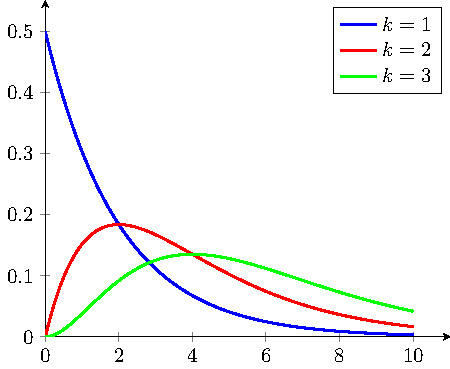
\includegraphics[width=0.8\textwidth]{Figures/chi-squared.pdf}
  \end{figure}
\end{minipage}

\begin{remark}
  Note that although \(X_i\) are independent \(\text{Normal}(\mu, \sigma)\), the variables \(X_i - \overline{X}\) are not independent. Suppose \(X_1 - \overline{X} = z_1, X_2 - \overline{X} = z_2\), then  
  \[
  z_1 + z_2 + \cdots + z_n = (X_1 + X_2 + \cdots + X_n) - n\overline{X} = 0.
  \]  
\end{remark}

\begin{theorem}
  If \(X_1, \cdots, X_n\) are independent random variables following \(\mathcal{N}(\mu, 1)\), then
  \[
    (X_1 - \overline{X})^2 + \cdots + (X_n - \overline{X})^2 \sim \chi^2(n - 1),
  \]
  where \(\overline{X} = \frac{1}{n}\sum_{i=1}^n X_i\) is the sample mean.
\end{theorem}

\begin{corollary}
  If \(X_1, \cdots, X_n\) are independent random variables following \(\mathcal{N}(\mu, \sigma^2)\), then
  \[
    \dfrac{(n - 1)S^2}{\sigma^2} \sim \chi^2(n - 1),
  \]
  where \(S^2 = \frac{1}{n - 1}\sum_{i = 1}^n (X_i - \overline{X})^2\) is the sample variance.
\end{corollary}


\(\circledast \) Then, to find the confidence interval for \(\sigma\), we have
\[
  \begin{aligned}
    \mathbb{P}(z^- \leq \chi^2(n - 1) \leq z^+) &= \mathbb{P}(z^- \leq \chi^2(n - 1) \leq z^+) \\
    &= \mathbb{P}(z^- \leq \frac{(n-1)S^2}{\sigma^2} \leq z^+) \\
    &= \mathbb{P}(\dfrac{(n - 1)S^2}{z^+} \leq \sigma^2 \leq \dfrac{(n - 1)S^2}{z^-}) \\
    &= \mathbb{P}(\sqrt{\dfrac{(n - 1)S^2}{z^+}} \leq \sigma \leq \sqrt{\dfrac{(n - 1)S^2}{z^-}}) \\
  \end{aligned}
\]


Now, we can go back to the discussion. 

\subsection{Student's \(t\) Random Variable}
Since we consider the case where \(\sigma\) is unknown, we can no longer use the previous method, i.e., \(\frac{\overline{X} - \mu}{\sigma / \sqrt{n}}\), to find the confidence interval for the mean. Instead, we use the sample variance \(S\) to estimate the confidence interval. However, in this case, the distribution is no longer normal.

For example, we have 
\[
    T = \frac{\overline{X} - \mu}{\frac{S}{\sqrt{n}}} = \dfrac{\text{Normal}(0, \frac{\sigma}{\sqrt{n}})}{\sqrt{\dfrac{\sigma^2 \chi^2(n - 1)}{n(n - 1)}}} = \dfrac{\text{Normal}(0, 1)}{\sqrt{\dfrac{\chi^2(n - 1)}{(n - 1)}}}
\]
Since \(\text{Normal}(0, 1)\) and \(\sqrt{\frac{\chi^2(n - 1)}{n - 1}}\) are independent, we can define a random variable for this distribution. This is what we call the Student's \(t\)-distribution.

If \(X_1, \cdots, X_n\) are independent random variables with distribution \(\mathcal{N}(\mu, \sigma^2)\), then a \((1 - \alpha)\)-confidence interval for the mean \(\mu\) is given by
\[
  \overline{x} \pm t_{\frac{\alpha}{2}} \dfrac{s}{\sqrt{n}},
\]
where \(t_{\frac{\alpha}{2}}\) is the \(t\)-score such that the area to the right of it under the \(t\)-distribution curve with \(n - 1\) degrees of freedom is \(\frac{\alpha}{2}\).

Consider two independent random variables \(Y\) and \(Z\), such that \(Y\) has the \(\chi^2\) distribution with \(n\) degrees of freedom \((\chi^2(n))\) and \(Z\) has the standard normal distribution \(\mathcal{N}(0, 1)\). Suppose a random variable \(T\) is defined as
\[
  T = \dfrac{Z}{\sqrt{\frac{Y}{n}}} = \dfrac{\mathcal{N}(0, 1)}{\sqrt{\frac{\chi^2(n)}{n}}}.
\]
The distribution of \(T\) is called the \(t\)-distribution or Student's \(t\)-distribution with \(n - 1\) degrees of freedom.

\begin{theorem}
  If \(X_1, \cdots, X_n\) are independent random variables following \(\mathcal{N}(\mu, \sigma^2)\), regardless of whether \(n\) is large or not, then we have
  \[
    T = \frac{\overline{X} - \mu}{\frac{S}{\sqrt{n}}} \sim t(n - 1),
  \]
  where \(\overline{X} = \frac{1}{n}\sum_{i = 1}^n X_i\) is the sample mean, and \(S^2 = \frac{1}{n - 1}\sum_{i = 1}^n (X_i - \overline{X})^2\) is the sample variance.
  
  \begin{proof}
    As \(X_1, \cdots, X_n\) are independent \(\mathcal{N}(\mu, \sigma^2)\) random variables, we have 
    \[
      Z = \dfrac{\overline{X} - \mu}{\frac{\sigma}{\sqrt{n}}} \sim \mathcal{N}(0, 1) \quad \text{and} \quad \dfrac{(n - 1)S^2}{\sigma^2} \sim \chi^2(n - 1)
    \]
    Denote \(Y = \dfrac{(n - 1)S^2}{\sigma^2} \sim \chi^2(n - 1)\). Then,
    \[
      T = \dfrac{Z}{\sqrt{\frac{Y}{n - 1}}} \sim t(n - 1) \Longleftrightarrow T = \dfrac{\frac{\overline{X} - \mu}{\frac{\sigma}{\sqrt{n}}}}{\frac{S}{\sigma}} = \dfrac{(\overline{X} - \mu)}{\frac{S}{\sqrt{n}}} \sim t(n - 1)
    \]
    This holds true when \(Z\) and \(Y\) are independent. 
  
    To show that \(Z\) and \(Y\) are independent, we prove that \(\overline{X}\) and \(S^2\) are independent. Since
    \[
      S^2 = \frac{1}{n-1} \sum_{i=1}^{n} (X_i - \overline{X})^2,
    \]
    it suffices to show that \(\overline{X}\) and \(X_i - \overline{X}\) are independent. We know that
    \[
      \overline{X} \sim \mathcal{N}\left(\mu, \dfrac{\sigma^2}{n}\right) \quad \text{and} \quad (X_i - \overline{X}) \sim \mathcal{N} \left(0, \frac{n - 1}{n} \sigma^2\right).
    \]
    We now calculate the covariance between \(\overline{X}\) and \(X_i - \overline{X}\):
    \[
      \begin{aligned}
        \Cov(\overline{X}, X_i - \overline{X}) &= \Cov(\overline{X}, X_i) - \Cov(\overline{X}, \overline{X}) \\
        &= \dfrac{1}{n}\Cov(X_i, X_i) - \Cov(\overline{X}, \overline{X}) \\
        &= \dfrac{\sigma^2}{n} - \dfrac{\sigma^2}{n} = 0.
      \end{aligned}
    \]
    Thus, \(\overline{X}\) and \(X_i - \overline{X}\) are independent, and therefore, \(Z\) and \(Y\) are independent.
  \end{proof}
  \end{theorem}
  

\begin{figure}[H]
  \centering
  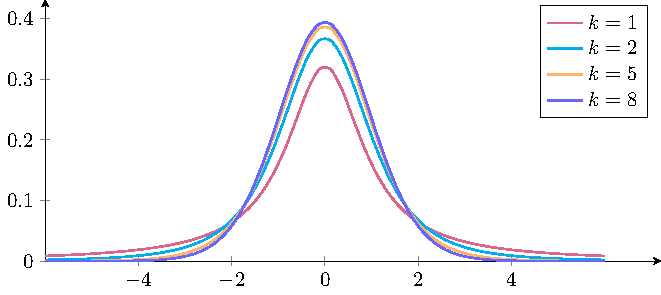
\includegraphics[width=0.6\textwidth]{Figures/t-dis.pdf}
\end{figure}

As shown in the graph, we can see that with a larger \(n\), the distribution becomes more similar to the standard normal distribution \(\mathcal{N}(0, 1)\), since the sample variance becomes a more accurate estimate of the population variance: 
\[
  t(n) = \dfrac{\mathcal{N}(0, 1)}{\sqrt{\frac{\chi^2(n)}{n}}} \overset{n \to \infty}{\Longrightarrow} \mathcal{N} (0, 1)
\]

Now, if \(X_1, \cdots, X_n\) are independent \(\mathcal{N} (\mu, \sigma^2)\), then a \((1 - \alpha)\)-confidence interval for the mean \(\mu\) is  
\[
  \overline{x} \pm t_{\frac{\alpha}{2}}\dfrac{s}{\sqrt{n}}
\]
where the \(t\)-value gives us the area to the right of it under the \(t\)-distribution curve with degrees of freedom \(n - 1\) equal to \(\frac{\alpha}{2}\).

\begin{proof}
  Given \(X_1, \cdots, X_n\) are independent random variables following \(\mathcal{N}(\mu, \sigma^2)\), where \(\sigma^2\) is unknown, and \(n\) is small (\(n < 30\)), we have
  \[
    T = \frac{\overline{X} - \mu}{\frac{S}{\sqrt{n}}} \sim t(n - 1).
  \]
  Therefore, the probability that \(T\) lies between the critical values \( \pm t_{\frac{\alpha}{2}} \) is
  \[
    \mathbb{P}\left(-t_{\frac{\alpha}{2}} \leq \dfrac{\overline{X} - \mu}{\frac{S}{\sqrt{n}}} \leq t_{\frac{\alpha}{2}}\right) = 1 - \alpha.
  \]
  By multiplying through by \(\frac{S}{\sqrt{n}}\), we get
  \[
    \mathbb{P}\left(-t_{\frac{\alpha}{2}}\frac{S}{\sqrt{n}} \leq \overline{X} - \mu \leq t_{\frac{\alpha}{2}}\frac{S}{\sqrt{n}}\right) = 1 - \alpha.
  \]
  Finally, solving for \(\mu\), we obtain the confidence interval for \(\mu\):
  \[
    \mathbb{P}\left(\overline{X} - t_{\frac{\alpha}{2}}\frac{S}{\sqrt{n}} \leq \mu \leq \overline{X} + t_{\frac{\alpha}{2}}\frac{S}{\sqrt{n}}\right) = 1 - \alpha.
  \]
\end{proof}

\begin{eg}
  5 random athletes are 152, 163, 188, 201, and 192 cm tall. Given a 95\% confidence interval for \(\mu\).

  \textbf{Solution:} 
  Here we have \(n = 5\), so the degrees of freedom are \(n - 1 = 4\). 
  
  \[
    \overline{x} = \dfrac{152 + 163 + 188 + 201 + 192}{5} = 179.2
  \]
  \[
    s = \sqrt{\dfrac{\sum_{i = 1}^5 (x_i - 179.2)^2}{4}} = 20.73 
  \]
  For \(\alpha = 5\%\), we have \(\frac{\alpha}{2} = 2.5\% = 0.025 \Rightarrow t_{\frac{\alpha}{2}} = 2.78\). 
  \[
    \overline{x} \pm t_{\frac{\alpha}{2}} \dfrac{s}{\sqrt{n}} = 179.2 \pm 2.78 \times \dfrac{20.73}{\sqrt{5}} = 179.2 \pm 25.78 \Rightarrow [153.43, 204.97]
  \]
\end{eg}

\subsection{One-sided Confidence Interval}
Consider \(X_1, \cdots, X_n\) as independent \(\mathcal{N}(\mu, \sigma^2)\) random variables, where \(\sigma^2\) is unknown and \(n < 30\). We have:

\textbf{Lower one-sided}: Find \(\hat{\theta}_n^{\min}\) such that \(\mathbb{P}(\mu \geq \hat{\theta}_n^{\min}) = 1 - \alpha\)
\[
  \mathbb{P}(T \leq t_{\alpha}) = \mathbb{P} \left(\dfrac{\overline{X} - \mu}{\frac{S}{\sqrt{n}}} \leq t_{\alpha}\right) = 1 - \alpha \Longrightarrow \mathbb{P}\left(\mu \geq \overline{X} - t_{\alpha}\dfrac{S}{\sqrt{n}}\right) = 1 - \alpha
\]
Given specific values of \(\overline{x}\) and \(s\), we have 
\[
  \left[\overline{x} - t_{\alpha}, +\infty\right]
\]

\textbf{Upper one-sided}: Find \(\hat{\theta}_n^{\max}\) such that \(\mathbb{P}(\mu \leq \hat{\theta}_n^{\max}) = 1 - \alpha\)
\[
  \mathbb{P}(T \geq -t_{\alpha}) = \mathbb{P} \left(\dfrac{\overline{X} - \mu}{\frac{S}{\sqrt{n}}} \geq t_{\alpha}\right) = 1 - \alpha \Longrightarrow \mathbb{P}\left(\mu \leq \overline{X} + t_{\alpha}\dfrac{S}{\sqrt{n}}\right) = 1 - \alpha
\]
Given specific values of \(\overline{x}\) and \(s\), we have 
\[
  \left[-\infty, \overline{x} + t_{\alpha}\right]
\]

\section{Summary}
In summary, if \(X_1, \cdots, X_n\) are independent samples with the same PMF or PDF, for a \((1 - \alpha)\)-confidence interval, we consider the following cases:

1. \textbf{Known \(\sigma^2\)}

If \(n\) is large, i.e. \(n \geq 30\), or if \(n < 30\) with the PDF \(\mathcal{N} (\mu, \sigma^2)\), we have:
\[
  Z = \dfrac{\overline{X} - \mu}{\frac{\sigma}{\sqrt{n}}} \sim \mathcal{N}(0, 1), \quad \overline{x} \pm z_{\frac{\alpha}{2}} \dfrac{\sigma}{\sqrt{n}}
\]

2. \textbf{Unknown \(\sigma^2\)}

\textbf{Case 1:} If \(n\) is large, then we have:
\[
  \sigma \approx s, \quad Z = \dfrac{\overline{X} - \mu}{\frac{s}{\sqrt{n}}} \sim \mathcal{N}(0, 1), \quad \overline{x} \pm z_{\frac{\alpha}{2}} \frac{s}{\sqrt{n}}
\]

\textbf{Case 2:} If \(n < 30\), with the PDF \(\mathcal{N} (\mu, \sigma^2)\), then we have:
\[
  T = \frac{\overline{X} - \mu}{\frac{S}{\sqrt{n}}} \sim t(n - 1), \quad \overline{x} \pm t_{\frac{\alpha}{2}} \frac{s}{\sqrt{n}}
\]
